% tikz/teaser.tex -- Figure 1 (input from sections/01_introduction.tex): (a) the routes of teacher B4 on
% MPS4 and binary4 (TikZ, below); (b, c) data panels drawn by experiments/report_figures/make_teaser.py.
% Sites are numbered from 0. Layout as in ttn/tree.py: MPS4 core i carries site i; binary4 has a root
% without sites and two leaf cores carrying sites 0, 1 and 2, 3. Orders checked in
% experiments/locality/results/levels_summary.csv (B4: mps4 0>1>2 in 60 runs, binary4 0>2>1 in 48).
\definecolor{teaserroute}{HTML}{762A83}
\tikzset{
  tzcore/.style={circle, draw=black!40, fill=white, line width=0.5pt, minimum size=3mm, inner sep=0pt},
  tzroute/.style={tzcore, draw=teaserroute, line width=0.9pt},
  tzcarry/.style={tzroute, fill=teaserroute!40},
  tzbond/.style={line width=0.8pt, black!30},
  tzrbond/.style={line width=2.2pt, teaserroute},
  tzleg/.style={line width=0.5pt, black!35},
  tzrleg/.style={line width=0.9pt, teaserroute},
  tzsite/.style={font=\tiny, inner sep=0.6pt, text=black!60},
  tzrsite/.style={tzsite, text=teaserroute, font=\tiny\bfseries},
  tznote/.style={font=\scriptsize, align=center, inner sep=1pt},
}
% One mini tree per (tree, component). Cores: tzcarry = carries a site where the component differs
% from 0000; tzroute = on the Steiner subtree only; tzcore = off the route.
\newcommand{\teaserpanel}{%
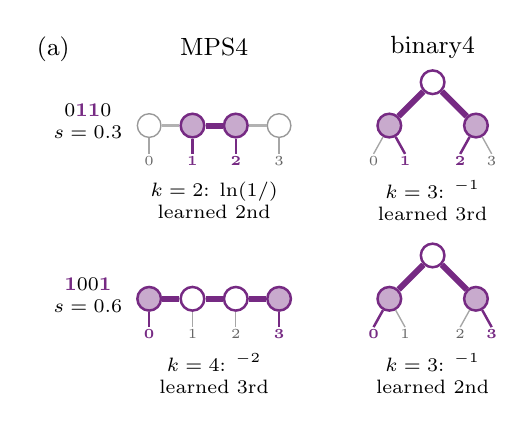
\begin{tikzpicture}[x=1cm, y=1cm]
  \node[font=\small, anchor=north west] at (-1.55, 1.25) {(a)};
  \node[tznote, font=\small] at (0.825, 1.0) {MPS4};
  \node[tznote, font=\small] at (3.6, 1.0) {binary4};
  % row 1: component 0110 (weight 0.3), differs on sites 1, 2
  \node[tznote, anchor=east] at (-0.3, 0.05)
    {$0\textcolor{teaserroute}{\mathbf{11}}0$\\ $s=0.3$};
  \node[tzcore] (a0) at (0, 0) {};    \node[tzcarry] (a1) at (0.55, 0) {};
  \node[tzcarry] (a2) at (1.1, 0) {}; \node[tzcore] (a3) at (1.65, 0) {};
  \draw[tzbond] (a0) -- (a1);  \draw[tzrbond] (a1) -- (a2);  \draw[tzbond] (a2) -- (a3);
  \draw[tzleg] (a0) -- ++(0,-0.36) node[tzsite, below] {0};
  \draw[tzrleg] (a1) -- ++(0,-0.36) node[tzrsite, below] {1};
  \draw[tzrleg] (a2) -- ++(0,-0.36) node[tzrsite, below] {2};
  \draw[tzleg] (a3) -- ++(0,-0.36) node[tzsite, below] {3};
  \node[tznote] at (0.825, -0.95) {$k=2$: $\ln(1/\isc)$\\ learned 2nd};
  \node[tzcarry] (b0) at (3.05, 0) {}; \node[tzcarry] (b1) at (4.15, 0) {};
  \node[tzroute] (br) at (3.6, 0.55) {};
  \draw[tzrbond] (b0) -- (br) -- (b1);
  \draw[tzleg] (b0) -- ++(-0.2,-0.36) node[tzsite, below] {0};
  \draw[tzrleg] (b0) -- ++(0.2,-0.36) node[tzrsite, below] {1};
  \draw[tzrleg] (b1) -- ++(-0.2,-0.36) node[tzrsite, below] {2};
  \draw[tzleg] (b1) -- ++(0.2,-0.36) node[tzsite, below] {3};
  \node[tznote] at (3.6, -0.95) {$k=3$: $\isc^{-1}$\\ learned 3rd};
  % row 2: component 1001 (weight 0.6), differs on sites 0, 3
  \begin{scope}[yshift=-2.2cm]
  \node[tznote, anchor=east] at (-0.3, 0.05)
    {$\textcolor{teaserroute}{\mathbf{1}}00\textcolor{teaserroute}{\mathbf{1}}$\\ $s=0.6$};
  \node[tzcarry] (c0) at (0, 0) {};    \node[tzroute] (c1) at (0.55, 0) {};
  \node[tzroute] (c2) at (1.1, 0) {};  \node[tzcarry] (c3) at (1.65, 0) {};
  \draw[tzrbond] (c0) -- (c1) -- (c2) -- (c3);
  \draw[tzrleg] (c0) -- ++(0,-0.36) node[tzrsite, below] {0};
  \draw[tzleg] (c1) -- ++(0,-0.36) node[tzsite, below] {1};
  \draw[tzleg] (c2) -- ++(0,-0.36) node[tzsite, below] {2};
  \draw[tzrleg] (c3) -- ++(0,-0.36) node[tzrsite, below] {3};
  \node[tznote] at (0.825, -0.95) {$k=4$: $\isc^{-2}$\\ learned 3rd};
  \node[tzcarry] (d0) at (3.05, 0) {}; \node[tzcarry] (d1) at (4.15, 0) {};
  \node[tzroute] (dr) at (3.6, 0.55) {};
  \draw[tzrbond] (d0) -- (dr) -- (d1);
  \draw[tzrleg] (d0) -- ++(-0.2,-0.36) node[tzrsite, below] {0};
  \draw[tzleg] (d0) -- ++(0.2,-0.36) node[tzsite, below] {1};
  \draw[tzleg] (d1) -- ++(-0.2,-0.36) node[tzsite, below] {2};
  \draw[tzrleg] (d1) -- ++(0.2,-0.36) node[tzrsite, below] {3};
  \node[tznote] at (3.6, -0.95) {$k=3$: $\isc^{-1}$\\ learned 2nd};
  \end{scope}
\end{tikzpicture}}
\begin{figure}[t]
  \centering
  \begin{minipage}[b]{0.415\textwidth}
    \centering\teaserpanel
  \end{minipage}\hfill
  \begin{minipage}[b]{0.56\textwidth}
    \centering\includegraphics[width=\textwidth]{intro/teaser.pdf}
  \end{minipage}
  \caption{The tree decides the later plateaus. (a)~Teacher B4: patterns $0000$ (weight $1$), $0110$ ($0.3$)
    and $1001$ ($0.6$), with local dimension $d=2$ and bond dimension $\chi=3$, on MPS4 (a chain of four
    cores, core $i$ carrying site $i$) and binary4 (two cores carrying sites $0,1$ and $2,3$, joined by a
    root without sites). Both trees learn $0000$ first. A remaining component then needs the cores that
    carry the sites where it differs from $0000$ (filled) and every core on the paths between them: its
    route, the Steiner subtree of those cores, with $k$ cores (outlined; its bonds in bold). The next
    plateau lasts $\propto\ln(1/\isc)$ for $k=2$ and $\propto\isc^{-(k-2)}$ for $k\ge3$, where $\isc$ is the
    initialization scale. On MPS4 the smaller component $0110$ ($k=2$) comes before $1001$ ($k=4$):
    locality beats weight. On binary4 both have $k=3$ and the larger comes first. Each order holds in every
    run (60 on MPS4, 48 on binary4); measured exponents $2.02\pm0.01$ on MPS4 and $1.05\pm0.01$,
    $1.03\pm0.01$ on binary4 (mean $\pm$ s.e.\ over $5$ and $8$ seeds). (b)~Loss of a run on MPS4 with an
    orthogonal teacher of weights $3,2,1$ ($d=4$, $\chi=3$, $\isc=0.01$; top left of \cref{fig:s2s-runs}): it
    rests at the partial-fit levels (dotted: the loss with $0$, $1$ or $2$ components learned) and drops by
    one component per escape. (c)~Plateau exponent after the first component against the prediction
    $k-2$: two-component teachers on nine trees, every case with $k=3$--$5$ (mean $\pm$ s.e.\ over up to
    eight seeds; filled: small initialization, open: started at the saddle). Larger $k$ and the slopes for
    $k=2$: \cref{fig:locality-exponents}. (source: App.~B, \cref{tab:exp-s2s,tab:exp-locality})}
  \label{fig:teaser}
\end{figure}
